\documentclass[UTF8,11pt]{ctexart}

\usepackage[margin=1in]{geometry}
\usepackage{booktabs}
\usepackage{graphicx}
\usepackage{amsmath}
\usepackage[hidelinks]{hyperref}
\usepackage{enumitem}
\usepackage{microtype}

\graphicspath{{figures/}}

\title{共享经验多智能体中的策略退化：迷宫机制实验草稿}
\author{实验小节中文稿}
\date{\today}

\begin{document}
\maketitle

\begin{abstract}
本文档整理当前 MazeEval-style 迷宫实验的阶段性结果。我们的核心问题不是“错误经验污染记忆”，而是更细的一类机制：一些局部上可行、文本上正确的策略，经过多智能体系统中的经验写入、共享检索和迭代复用后，被正反馈不断放大，最终导致全局低效、路线同质化，以及没有明显报错的循环行为。当前 pilot 结果显示，共享经验本身并不一定有害；reviewer 写入的共享经验在短迭代下可以提升表现。但当少量 direct/oracle 风格经验被高度集中地检索时，系统会出现更高的路径成本、更高的循环率，以及在更长反馈链条下的成功率崩溃。
\end{abstract}

\section{实验目标}

本实验想验证一个机制命题：多智能体共享经验系统中，局部可行策略是否会在共识写入、共享检索和反复复用中被放大成全局退化。这里的“退化”不是指 agent 学到了一条明显错误的知识，而是指它学到的经验文本本身可能是合理的，例如“尽量减少到目标的距离”“避免重复访问”“到达终点后立即提交”。问题在于，这些经验脱离了来源轨迹的上下文和质量信息后，可能被多个 agent 反复检索，最终让系统进入低效探索或循环。

迷宫环境适合作为机制显微镜。因为迷宫里可以严格区分“是否合法移动”“是否到达终点”“实际路径相对最短路径有多绕”。如果一个 agent 没有穿墙，也没有错误提交，而是合法移动了很久才成功，甚至在局部区域反复绕圈，这就对应我们想研究的 ant-mill 式策略退化。

\section{Benchmark 设计}

我们实现了一个 MazeEval-style 的可控迷宫环境，而不是让模型一次性看到完整地图并输出完整路径。每一步，agent 只能看到局部 observation，包括当前位置、目标位置、可走方向、四个方向到墙的距离、最近路径、已经访问过的位置、当前状态下尝试过的方向，以及检索到的经验。agent 不看到隐藏图结构，也不看到最短路径。

环境负责执行动作语义。模型如果试图撞墙，环境会阻止移动并记录 invalid move；只有在 goal cell 提交才算成功。因此 reviewer 或 evaluator 不会因为模型声称成功就直接判定成功，所有路线都由环境真实执行。当前 pilot 使用 $15 \times 15$ trap-family 迷宫，并要求最短路径长度至少为 30。heldout 迷宫在同一个 seed 下固定，方便不同 condition 在同一批任务上横向比较；train 迷宫用于产生经验写入。

\section{经验提炼与收集机制}

这一节需要单独说明，因为它决定本实验是不是一个玩具实验。我们的经验模块不是为迷宫专门手写一套坏规则，而是采用当前经验学习 agent 中常见的轨迹反思范式：参考 ExpeL 和 Reflexion 的做法，在 episode 结束后，把执行日志、成功失败和质量信号压缩成可迁移的自然语言经验；在多 agent 设置下，则采用 MAEL-like 的组织方式，让多个 agent 的轨迹可以进入私有经验池或共享经验池。迷宫环境只扮演 task adapter 的角色：它负责把轨迹、局部 observation 和质量字段格式化给通用经验提炼器，而不是直接生成某张迷宫的答案。

每条经验被写成简短的 \emph{do/avoid} 策略规则。经验提炼器会对比成功轨迹和低效轨迹，总结策略层面的经验，例如“如果回退后再次来到同一岔路，应优先选择尚未尝试的开放方向”。但它不能写 maze id、坐标、完整路径、固定动作序列，也不能把某次任务的答案缓存成经验。实现上，经验写入前还会经过 sanitizer，过滤坐标式文本、过长方向序列和过度具体的 episode 标识，保证经验池存的是抽象策略，而不是路线答案。

在 single-agent ExpeL calibration 中，一个 solver agent 在训练迷宫上产生轨迹，reviewer 只根据这个 agent 自己的日志写入经验。这个条件用于确认：在引入多 agent 共享之前，经验学习机制本身在迷宫家族中是否有用或至少可测。在 MAS 条件中，多个同构 solver agent 在同一迷宫的独立副本里行动；reviewer 只能看到 agent 的执行日志和质量摘要，例如 success、steps、invalid moves、revisits、stagnation 和 loop flags，而不能看到隐藏地图或求解路径。private memory 条件把每个 agent 的经验写回自己的经验池；shared memory 条件则把多个 agent 的经验合并到全局经验池，并在后续 episode 中共同检索。

direct 和 oracle 写入模式是消融实验，不是本文声称的主流 MAS 机制本体。它们的作用是隔离一个更纯粹的问题：当少数“文本上正确”的抽象策略被全局共享并高频检索时，系统是否会出现路线同质化、效率下降和循环。每条经验都会进入 memory audit，记录来源 episode、写入方式、support count、retrieval count 和后续影响过的 episode。这样我们可以区分“经验文本是否正确”和“这条经验来自什么样的轨迹、被怎样反复使用”这两个问题。

\section{实验条件}

\begin{description}[leftmargin=2.6cm, style=nextline]
    \item[Frozen] 写入经验，但不检索经验。这是“只存储、不注入”的控制组，用来确认变化不是由单纯存储造成的。
    \item[Private fixed] 每个 agent 只使用自己的私有经验池，不共享给其他 agent。这个条件用来测试经验是否有帮助，同时避免全局共享带来的正反馈。
    \item[Shared reviewer] reviewer 根据 agent 轨迹总结自然语言经验，并写入共享经验池。这是当前最接近主流 MAS 经验总结机制的条件。
    \item[Shared direct] 从轨迹结果中直接写入少量抽象策略，并全局共享。这个条件容易形成少数经验被反复检索。
    \item[Shared oracle] 根据成功或 oracle-style 评价写入共享经验。经验内容通常是正确的，但仍可能因为检索过度集中而诱发退化。
\end{description}

\section{指标}

主要指标包括成功率、路径成本、循环率、路线多样性、经验池大小和检索集中度。路径成本定义为
\[
    \mathrm{cost\_ratio} = \frac{\mathrm{actual\_steps}}{\mathrm{shortest\_path\_length}}.
\]
最短路径只用于研究者评估，不提供给 agent 或 reviewer。循环率用于刻画 agent 是否进入短周期位置循环或高重复访问状态。路线多样性用于观察多个 agent 的路线是否逐渐同质化。检索集中度用于衡量多个 agent 是否越来越依赖同几条经验。

\section{主实验矩阵：短反馈链下的经验学习}

表~\ref{tab:full-matrix-zh} 是 $T=3$、三个 seed 的五条件矩阵最终轮均值。Frozen 组非常稳定，因为它写经验但不检索。Private fixed 在成功率和成本上接近 frozen，同时保留了更高路线多样性。Shared reviewer 在短反馈链下表现最好：成功率达到 1.000，路径成本最低，循环率也最低。不过它的路线多样性最低，说明它确实会把 agent 的行为压缩到更同质的路线。Shared direct 和 shared oracle 则有更高的检索集中度，并表现出明显更高的路径成本。

\begin{table}[h]
\centering
\caption{$T=3$ 五条件矩阵最终轮均值，三个 seed 平均。}
\label{tab:full-matrix-zh}
\begin{tabular}{lrrrrrr}
\toprule
Condition & Success & Cost & Loop & Diversity & Memory & Retrieval conc. \\
\midrule
Frozen          & 0.944 & 2.334 & 0.056 & 0.177 & 8.0  & 0.000 \\
Private fixed   & 0.972 & 2.348 & 0.056 & 0.232 & 31.3 & 0.051 \\
Shared reviewer & 1.000 & 2.179 & 0.028 & 0.139 & 8.0  & 0.206 \\
Shared direct   & 0.917 & 3.092 & 0.139 & 0.277 & 1.7  & 0.804 \\
Shared oracle   & 0.944 & 3.042 & 0.083 & 0.236 & 2.0  & 0.783 \\
\bottomrule
\end{tabular}
\end{table}

\begin{figure}[h]
\centering
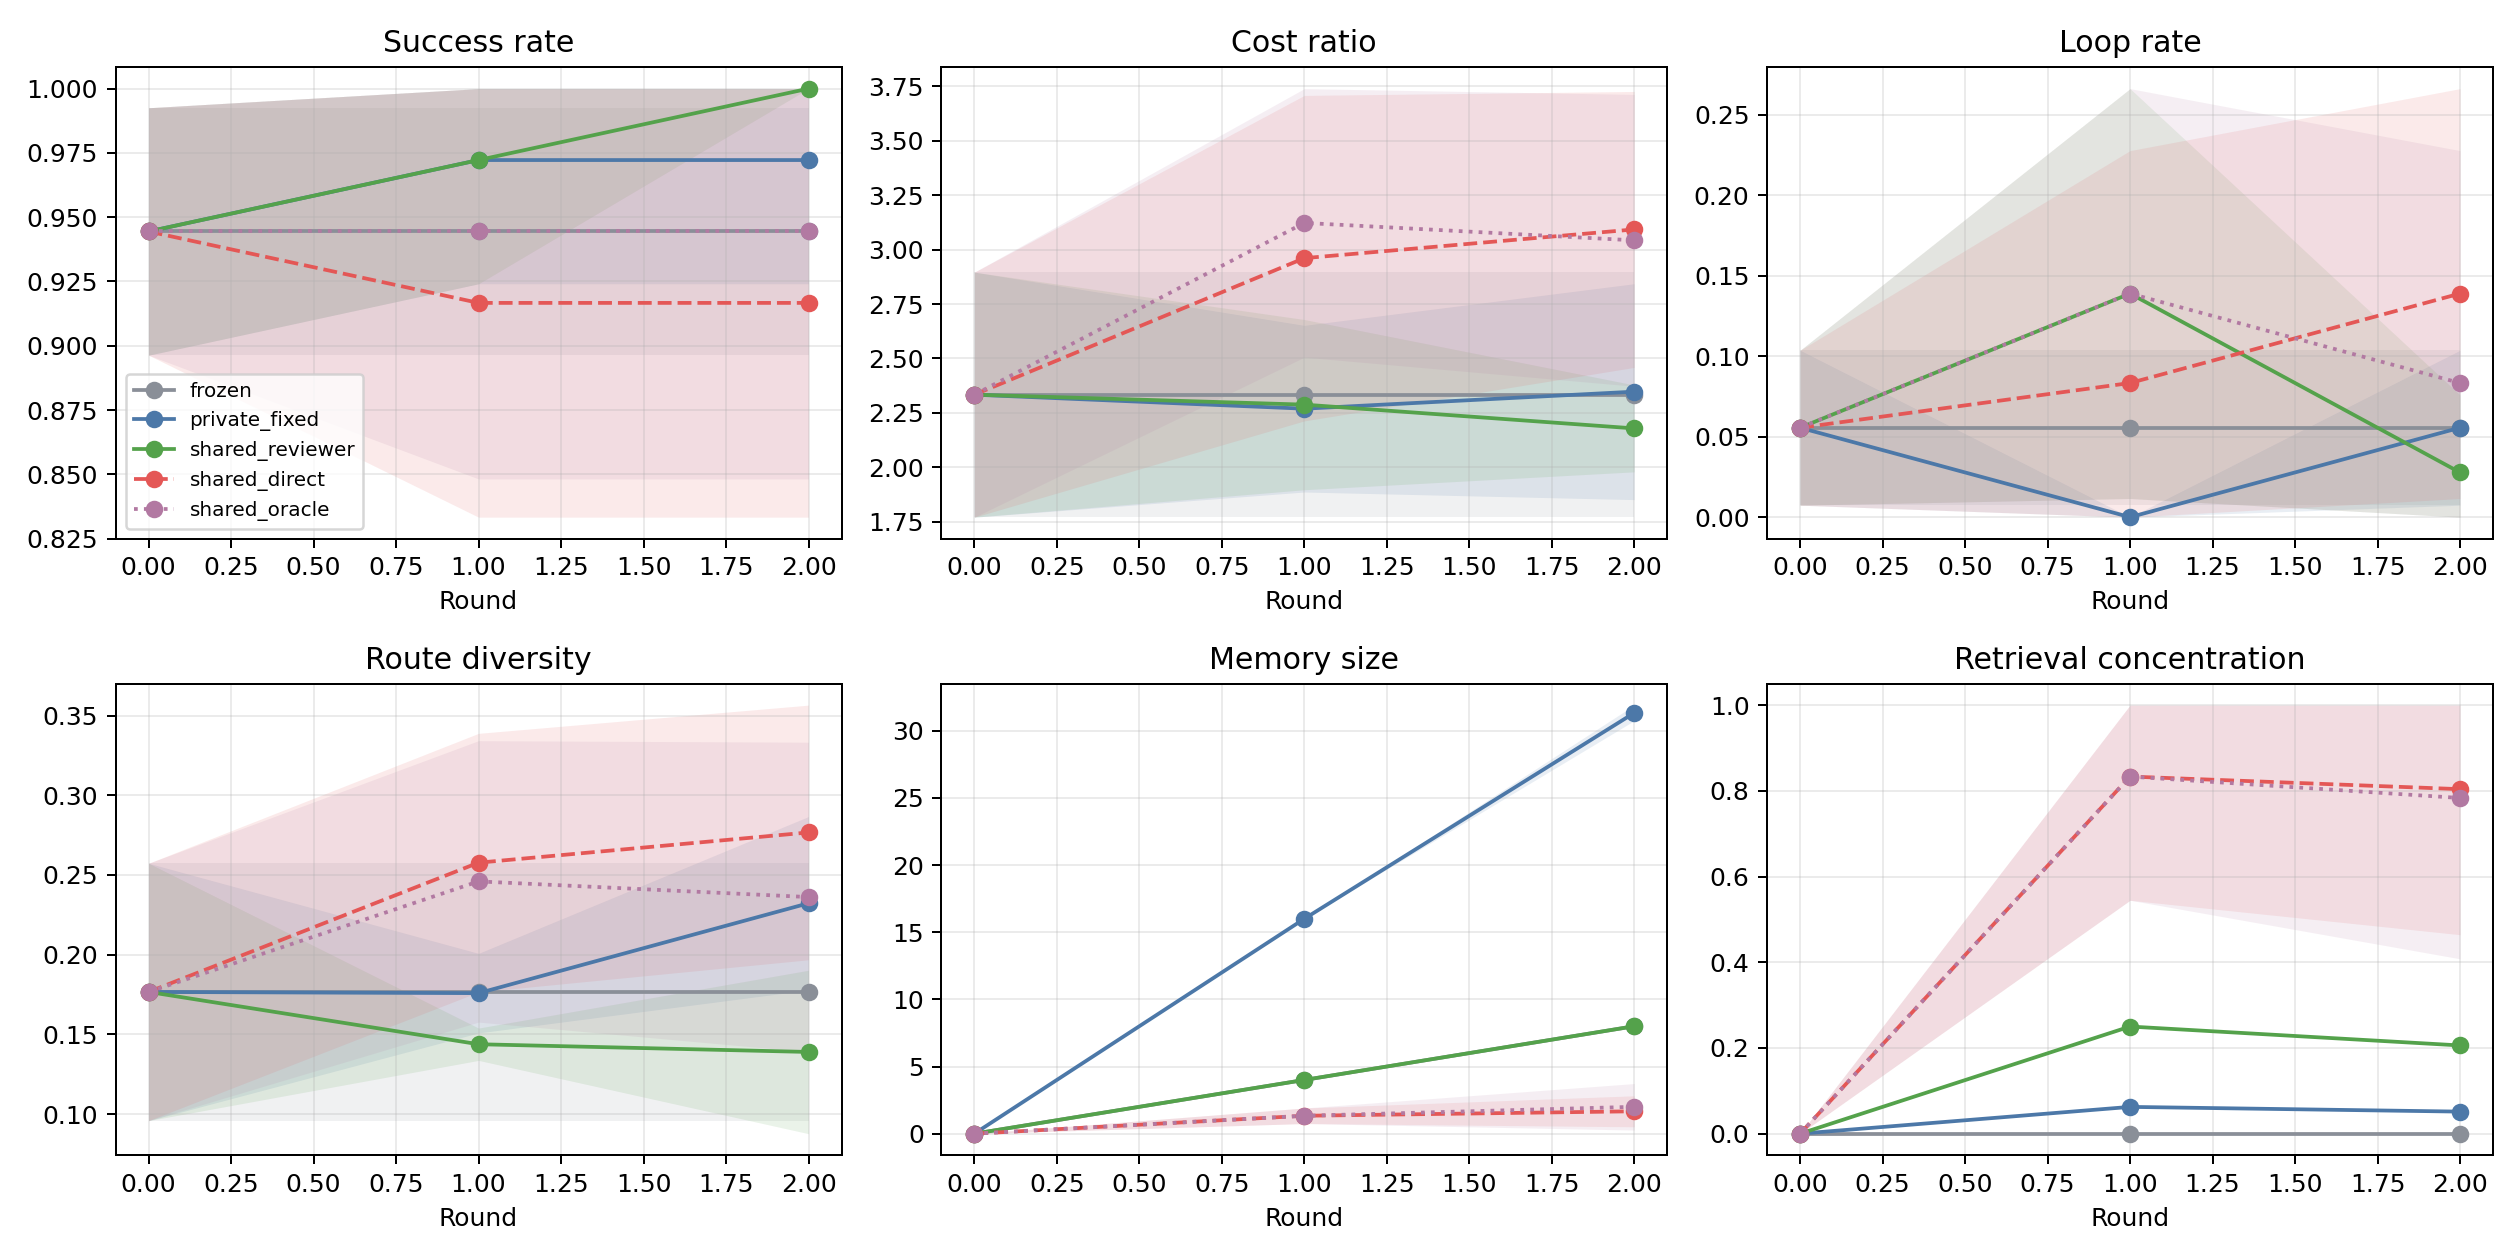
\includegraphics[width=\linewidth]{full_matrix_curves.png}
\caption{$T=3$ 完整矩阵。Shared reviewer 在短迭代下提升表现但压缩路线多样性；direct/oracle 经验带来更高 cost 和更高检索集中度。}
\label{fig:full-matrix-zh}
\end{figure}

\section{机制统计：检索集中度与 provenance}

机制分析支持一个更具体的解释：真正危险的不是“有经验”，而是少数经验被高度集中地反复检索。在 active-memory 轮次中，检索集中度与 cost ratio 的 Pearson 相关为 $r=0.663$，与 stagnation rate 的相关为 $r=0.646$，与 loop rate 的相关为 $r=0.349$。这说明，当系统越来越依赖少数共享经验时，路线成本和停滞程度会上升。

\begin{figure}[h]
\centering
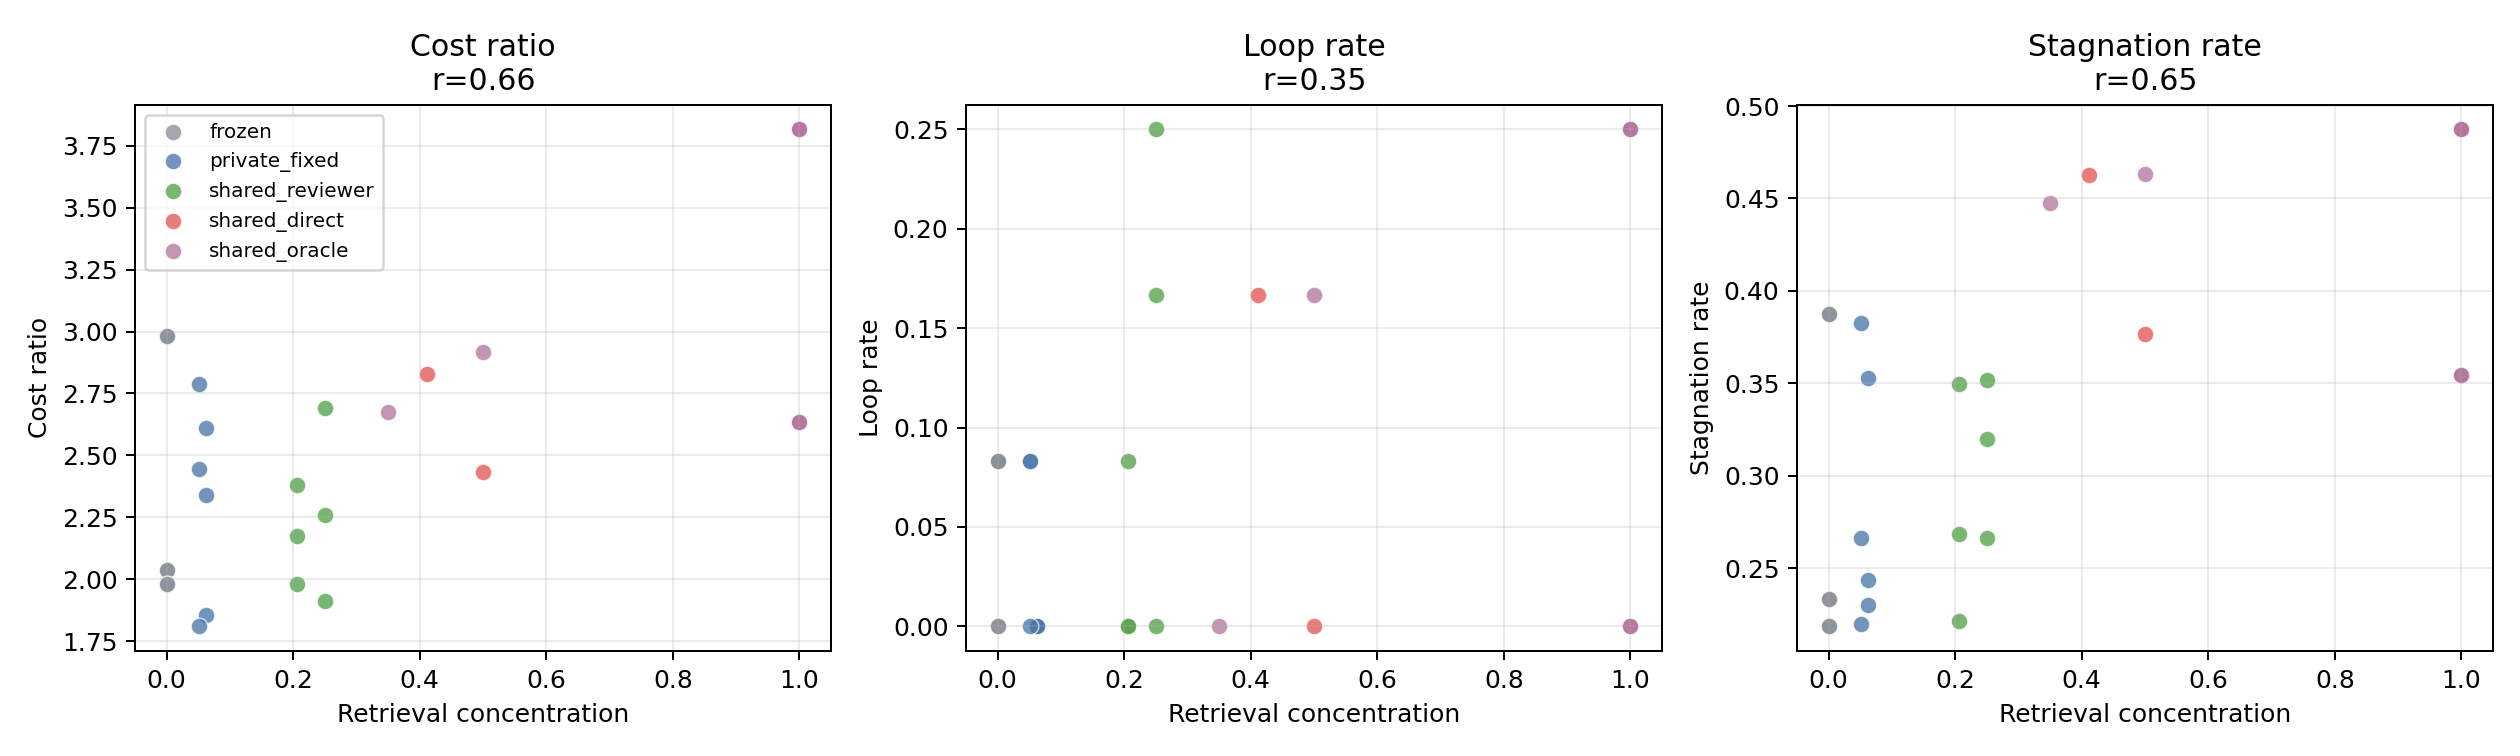
\includegraphics[width=\linewidth]{mechanism_scatter.png}
\caption{检索集中度与 cost/stagnation 呈正相关。每个点对应一个 condition/seed/round。}
\label{fig:mechanism-scatter-zh}
\end{figure}

provenance 审计进一步说明，经验文本正确不代表经验来源优质。最高频的 direct/oracle 经验通常是类似“减少到目标距离，避免重复访问，到达终点后立即提交”这样的正确陈述。但这些经验可能来自非常低效的轨迹：有些 source trajectory 的 cost 超过 5，有些甚至来自失败或高度停滞的 episode。因此，经验文本在被压缩成一句话后，丢失了“这条策略来自怎样的轨迹”这一关键信息。

\begin{figure}[h]
\centering
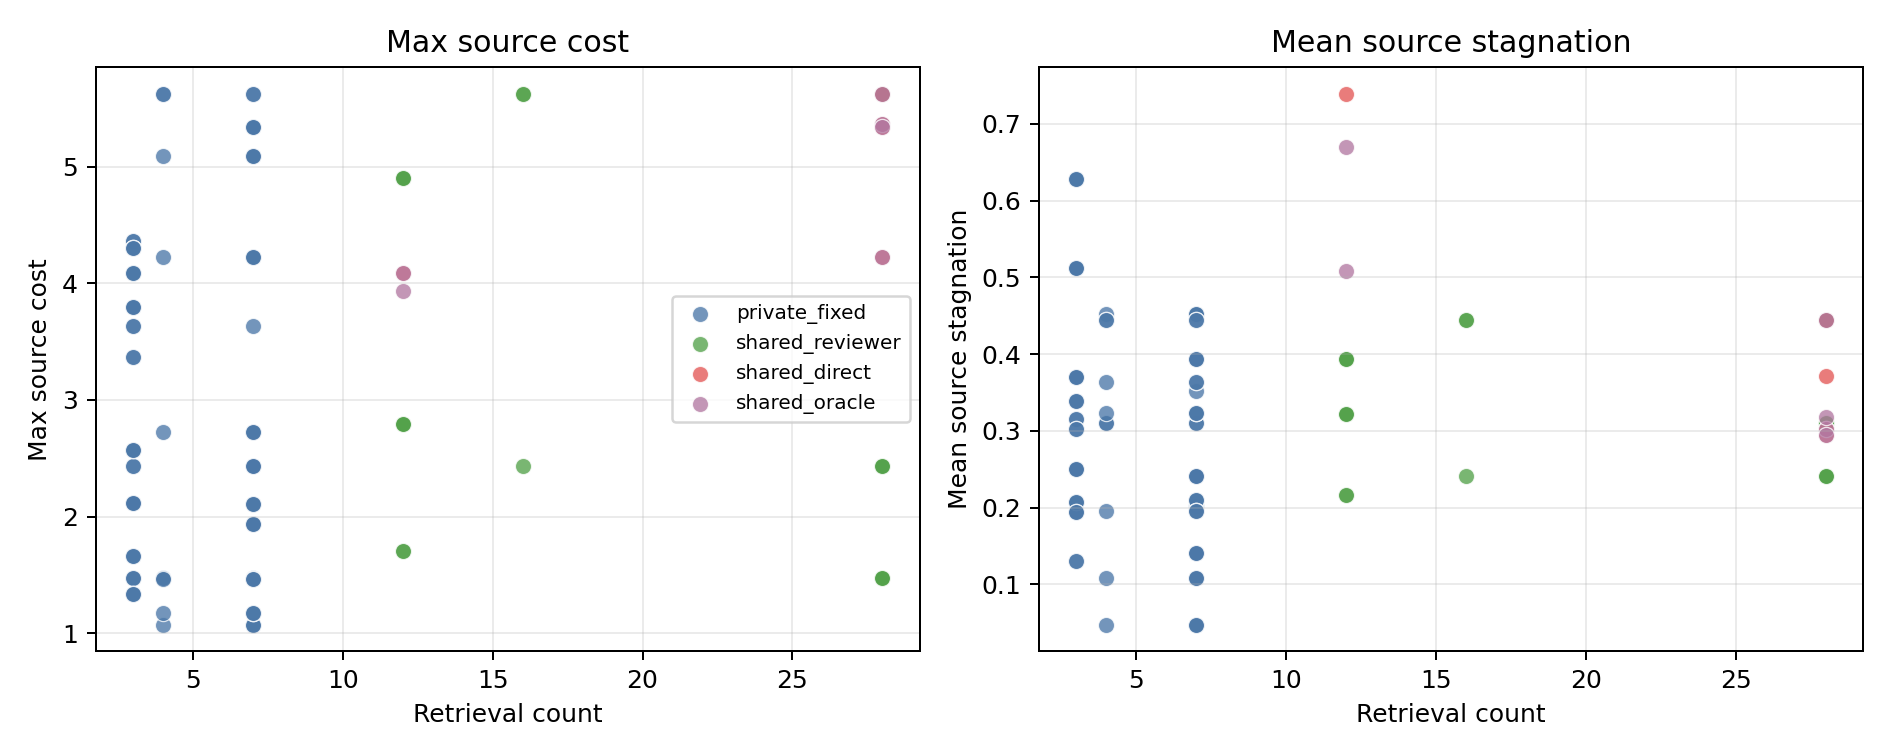
\includegraphics[width=0.86\linewidth]{provenance_scatter.png}
\caption{高频经验可能有较差 provenance。direct/oracle 经验被大量检索，但它们的来源轨迹可能 cost 很高或 stagnation 很高。}
\label{fig:provenance-zh}
\end{figure}

\section{更长反馈链：T=5 targeted stress}

为了测试退化是否会随着经验循环加深而暴露，我们做了 $T=5$ targeted stress，只保留 frozen、shared reviewer 和 shared direct 三组。Frozen 组在所有轮次里基本不变。Shared reviewer 在 $t=1$ 和 $t=2$ 确实改善了表现，但到 $t=3$ 和 $t=4$ 出现回退：cost 从 2.381 上升到 3.239，loop rate 上升到 0.167。Shared direct 的崩溃最明显：到 $t=4$，成功率降到 0.500，cost 升到 4.135，loop rate 达到 0.917。

\begin{table}[h]
\centering
\caption{$T=5$ targeted stress 的最终轮结果，seed 0。}
\label{tab:t5-zh}
\begin{tabular}{lrrrrrr}
\toprule
Condition & Success & Cost & Loop & Diversity & Memory & Retrieval conc. \\
\midrule
Frozen          & 0.917 & 2.982 & 0.083 & 0.264 & 15.0 & 0.000 \\
Shared reviewer & 0.917 & 3.239 & 0.167 & 0.257 & 15.0 & 0.183 \\
Shared direct   & 0.500 & 4.135 & 0.917 & 0.271 & 3.0  & 0.714 \\
\bottomrule
\end{tabular}
\end{table}

\begin{figure}[h]
\centering
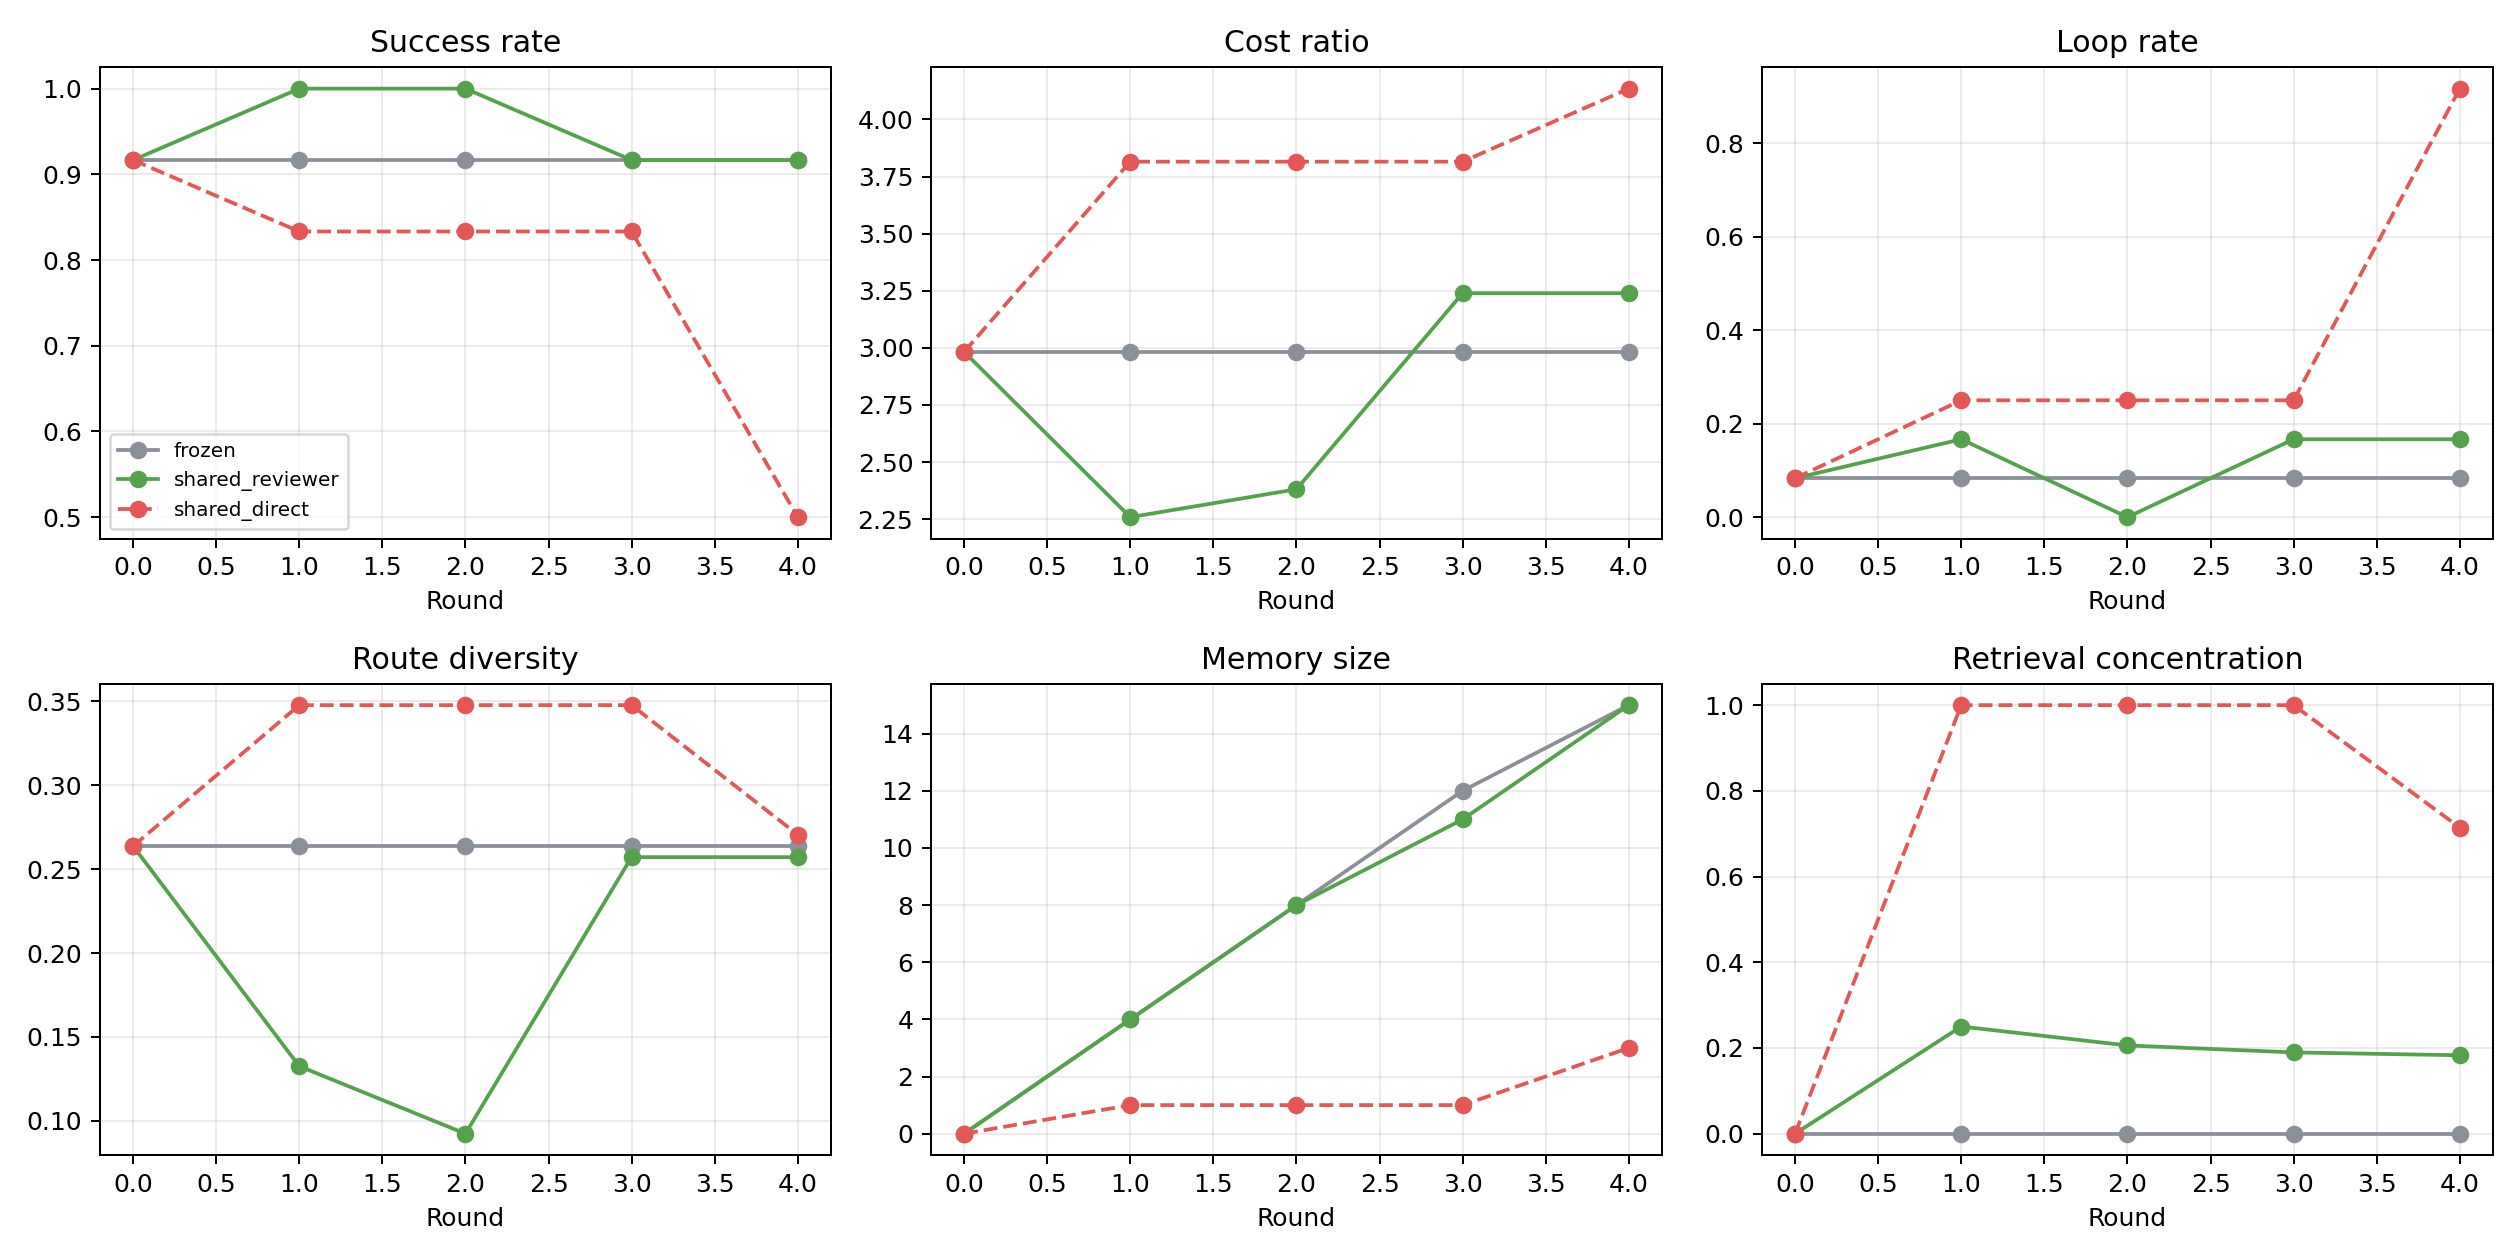
\includegraphics[width=\linewidth]{targeted_t5_curves.png}
\caption{$T=5$ stress test 暴露了更长反馈链下的策略退化。Shared direct 从低效复用进一步发展成高 loop collapse；shared reviewer 也在更多经验迭代后失去早期优势。}
\label{fig:t5-curves-zh}
\end{figure}

\section{案例：无报错的 ant-mill 式循环}

图~\ref{fig:t5-case-zh} 展示了 $T=5$ 中一个典型案例：同一张 heldout maze，round 4，agent 2，最短路径长度为 30。Frozen 组 67 步成功，没有 loop。Shared reviewer 79 步成功，没有 loop。Shared direct 最终也成功了，但用了 148 步，cost ratio 为 4.93，revisit maximum 为 34，stagnation rate 为 0.736，并被标记为 looped。

这个案例非常符合我们想表达的“无报错退化”：agent 没有穿墙，没有错误提交，也不是因为学到假知识而失败；它是在合法移动中不断绕路和重复访问，最后虽然完成了任务，但已经形成了类似 ant mill 的全局低效循环。

\begin{figure}[h]
\centering
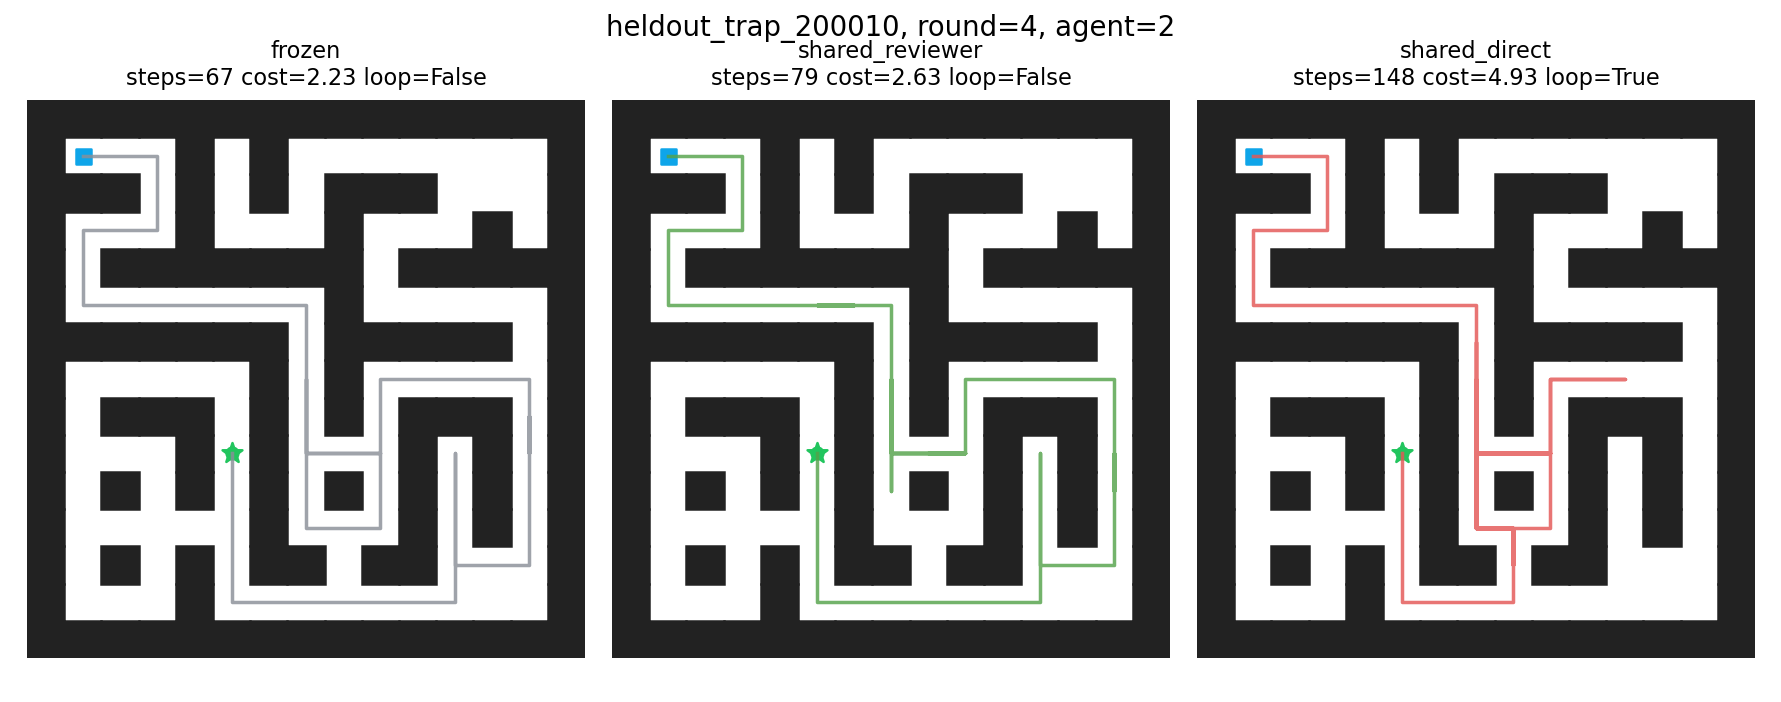
\includegraphics[width=\linewidth]{targeted_t5_case.png}
\caption{$T=5$ 机制案例。Shared direct 在 30 步最短路径的迷宫中走了 148 步，revisit maximum 为 34，并出现 loop。}
\label{fig:t5-case-zh}
\end{figure}

\section{阶段性解释}

目前结果可以支持四个初步判断。第一，共享经验不是天然有害，reviewer 写入的共享经验在短反馈链下可以提升表现。第二，direct/oracle 风格的少量共享经验即使文本正确，也可能因为检索过度集中而导致效率退化。第三，检索集中度是一个重要机制变量，它和 cost、stagnation 有明显正相关。第四，反馈链越长，越容易暴露短实验看不到的问题：$T=3$ 时 reviewer 看起来很稳，但 $T=5$ 时也开始出现后期退化。

这正好对应 ant-mill 类比：蚂蚁并不是学到了一条假规则，而是在局部合理的轨迹跟随中形成了全局死亡循环。我们的 MAS 设置中，agent 也不一定需要错误经验；局部可行策略被共享经验系统过度放大后，就可能变成全局低效甚至循环。

\section{局限与下一步}

这仍然是 pilot，而不是最终 benchmark。$T=3$ 矩阵目前有三个 seed，但 heldout 数量较小；$T=5$ stress 目前只有 seed 0。下一步需要补更多 seed，并把机制迁移到工具调用或网页任务中。在真实任务里通常没有最短路径，但可以用 task success、step count、tool calls、token cost、重复状态/动作、stagnation 和 time-to-success 来替代迷宫中的 cost ratio。

另外，后续还应该测试缓解方法，例如 provenance-aware retrieval、限制单条经验的检索支配度、鼓励 memory diversity，以及要求 reviewer 在写经验时显式惩罚高 cost source trajectory。这样可以把论文从“发现问题”推进到“解释问题并提出初步解决方向”。

\end{document}
